\documentclass{beamer}
% AnnArbor  Antibes  Bergen  Berkeley  Berlin  Boadilla  CambridgeUS  Copenhagen  Darmstadt  Dresden  Frankfurt  Goettingen  Hannover  Ilmenau  JuanLesPins  Luebeck  Madrid  Malmoe  Marburg  Montpellier  PaloAlto  Pittsburgh  Rochester  Singapore  Szeged  Warsaw  boxes  default 
\mode<presentation>
    {
      \usetheme{PaloAlto}
      \setbeamercovered{transparent}
    }
    \usepackage[english]{babel}
    \usepackage[latin1]{inputenc}
    \usepackage{times}
    \usepackage[T1]{fontenc}

%    \usepackage{graphicx}           
%    \usepackage{xeCJK}       
%    \usepackage{fontspec}
%    \setsansfont{SimSun}

    \title[A Brief Introduction to SDDS] {Case Study in Specification-Level Defects Detection}
    \subtitle{}
    \author[Author]{Jipeng Wu}
    \institute[Universities of Somewhere and Elsewhere] {
                                 Software Institute\\
                                 Nanjing University
     }
                               
\date[2014]
{Casual Presentation, 2014}

\subject{Theoretical Computer Science}
\AtBeginSubsection[]
{
  \begin{frame}<beamer>{Outline}
    \tableofcontents[currentsection,currentsubsection]
  \end{frame}
}
%========================================================================================================
\begin{document}

\begin{frame}
  \titlepage
\end{frame}

\begin{frame}{Outline}
  \tableofcontents
\end{frame}


\section{Our Purpose}
\begin{frame}{Code→Specification→Statecharts→Model Checking→Existence Proof}
  \begin{enumerate}
  \item 2 types of defects in codes:
    \begin{itemize}
    \item specification defects \pause
    \item implementation defects \pause
    \end{itemize}
  \item find a method to detect specification defects  \pause
  \item prove their existence in current open source projects \pause
  \end{enumerate}
\end{frame}

\section{Our Proposal}
\subsection{How we can specify a class?}
\begin{frame}{std def}
  \begin{enumerate}
  \item  A transition system is defined as a tuple (Q, l, R). \pause
  \item  Q is the set of states, usually specified by assignments of values to a set ofvariables V; \pause
  \item  l is a set of states (expressed as predicates on V ) defining the initial set of states; \pause
  \item  R is the transition relation, usually expressed by predicates containing unprimed and primed variables from V for the pre- and post-state. 
  \end{enumerate}
\end{frame}
\begin{frame}{state explosion}
  \begin{itemize}
  \item A flat representation means state explosion. \pause
  \item Hierarchy \pause
    \begin{figure}
      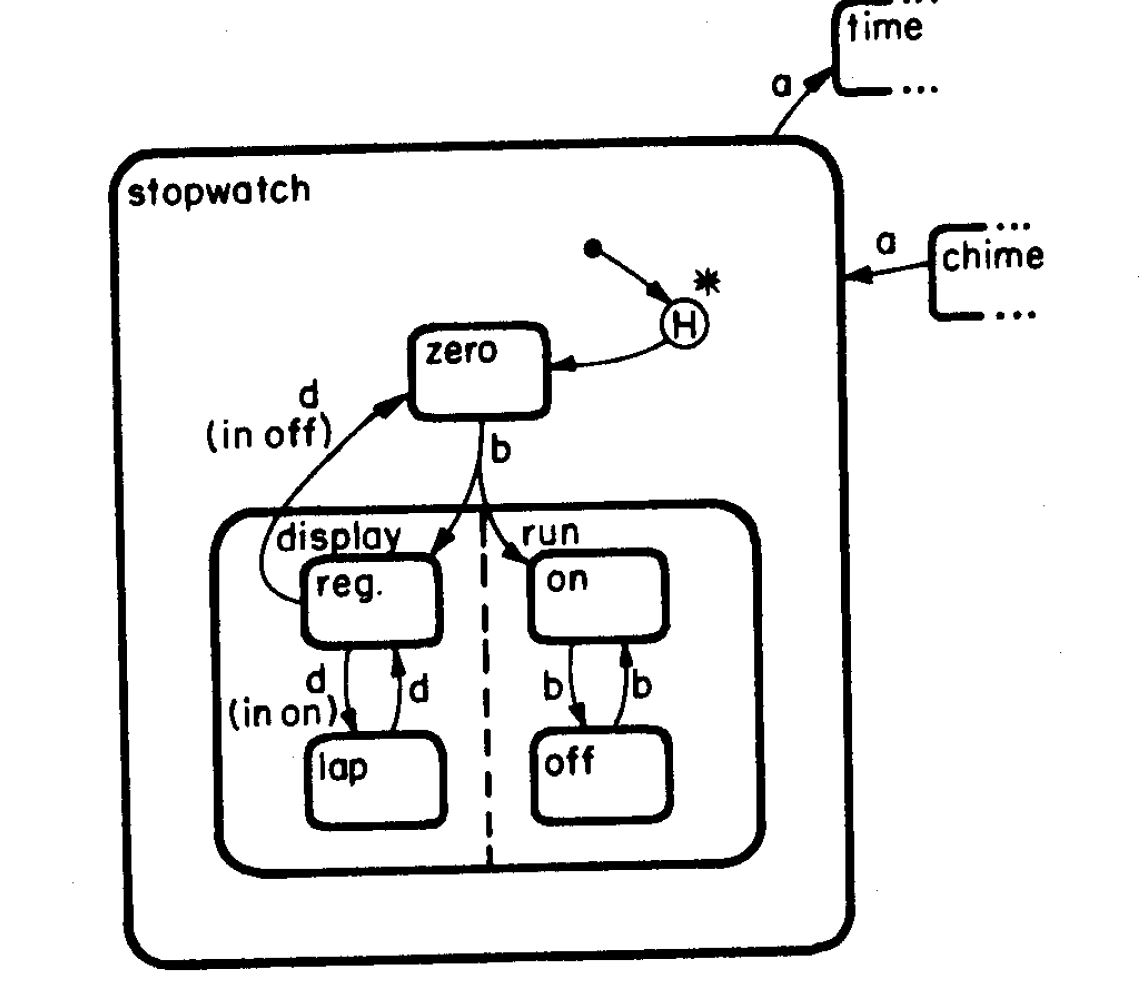
\includegraphics[width=2.4in]{img/1.JPG}
      \caption{A sample statecharts with hierarchy}
    \end{figure}
  \end{itemize}
\end{frame}

\subsection{How can we specify a class from its source code?}
\begin{frame}{Difficulty in Reversing Process}
  \begin{enumerate}
  \item The hierarchy is invisible for us. \pause
  \item We can get a flat representation. \pause
    \begin{figure}
      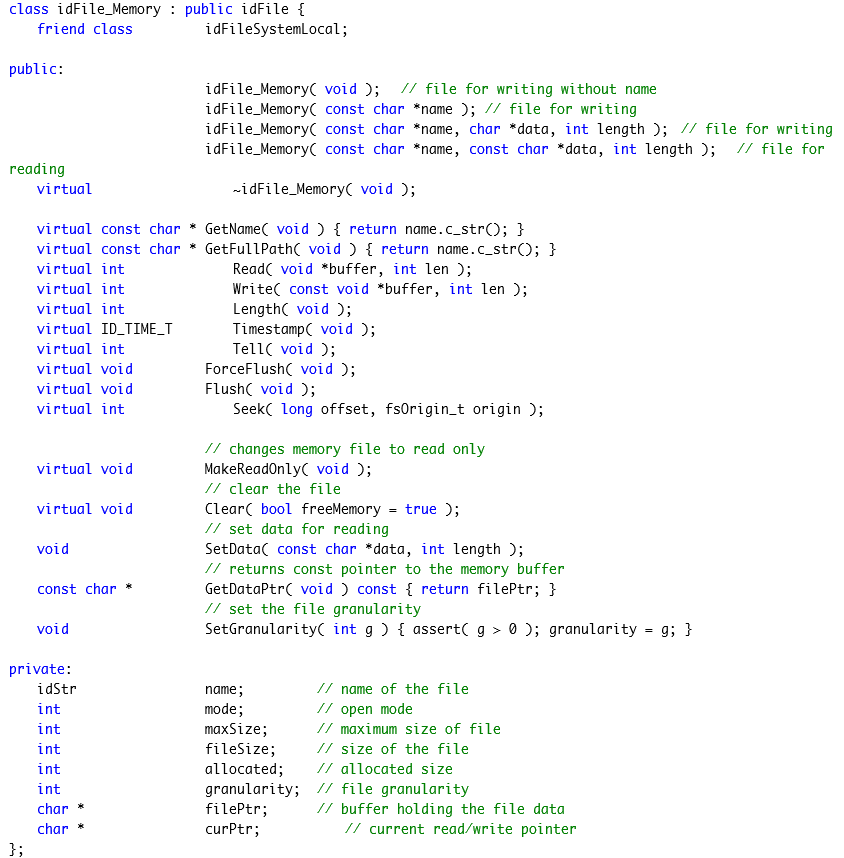
\includegraphics[width=2.4in]{img/2.PNG}
      \caption{A sample code}
    \end{figure}
  \item We need to reduce nr states by defining hirarchy reasonably.
  \end{enumerate}
\end{frame}

\begin{frame}{How to define a hirarchy?}
  Our Solution is called Specification Defects Detection Using Statecharts. \pause
  \begin{enumerate}
  \item Find out candidate state variables  \pause
  \item Find out methods with side effects \pause
  \item Elicit SDDS Clauses \pause
    \begin{enumerate}
    \item includes candidate state variables.
    \item The code executed when the clause is satisfied should contain changes to candidate state variables.
    \end{enumerate}
  \item	Convert SDDS Clauses to pre-states \pause
  \end{enumerate}
\end{frame}
\begin{frame}
  \begin{enumerate}
  \item Combine or separate pre-states and rename them \pause
  \item Determine initial states \pause
  \item Determine the function-level specifications. \pause
  \item Generate Statecharts. \pause
  \item Statecharts Checking. 
  \end{enumerate}
\end{frame}

\begin{frame}{Elicit SDDS Clauses}
      \begin{figure}
      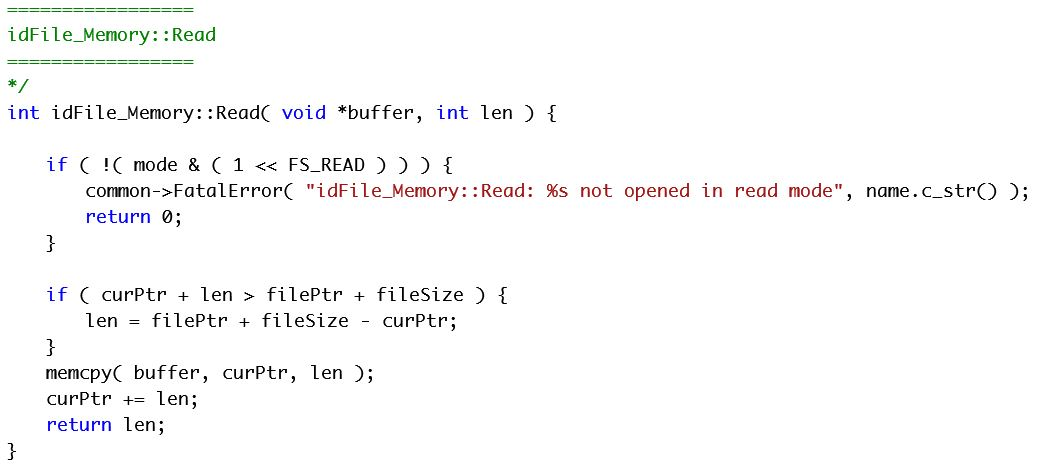
\includegraphics[width=2.4in]{img/3.JPG}
      \end{figure}
      \begin{figure}
      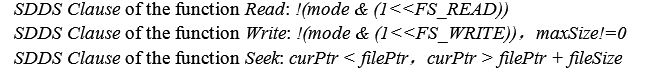
\includegraphics[width=2.4in]{img/4.JPG}
      \end{figure}
\end{frame}
\begin{frame}{Elicit Pre-states from SDDS Clauses}
  \begin{figure}
    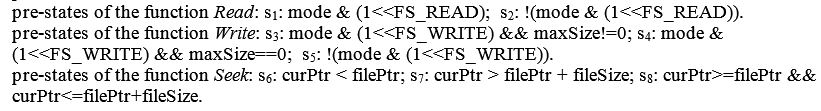
\includegraphics[width=3.0in]{img/5.JPG}
  \end{figure}
\end{frame}
\begin{frame}{Combine prestates}
  \begin{figure}
    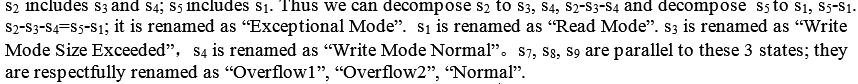
\includegraphics[width=3.0in]{img/6.JPG}
  \end{figure}
\end{frame}
\begin{frame}{Statecharts}
  \begin{figure}
    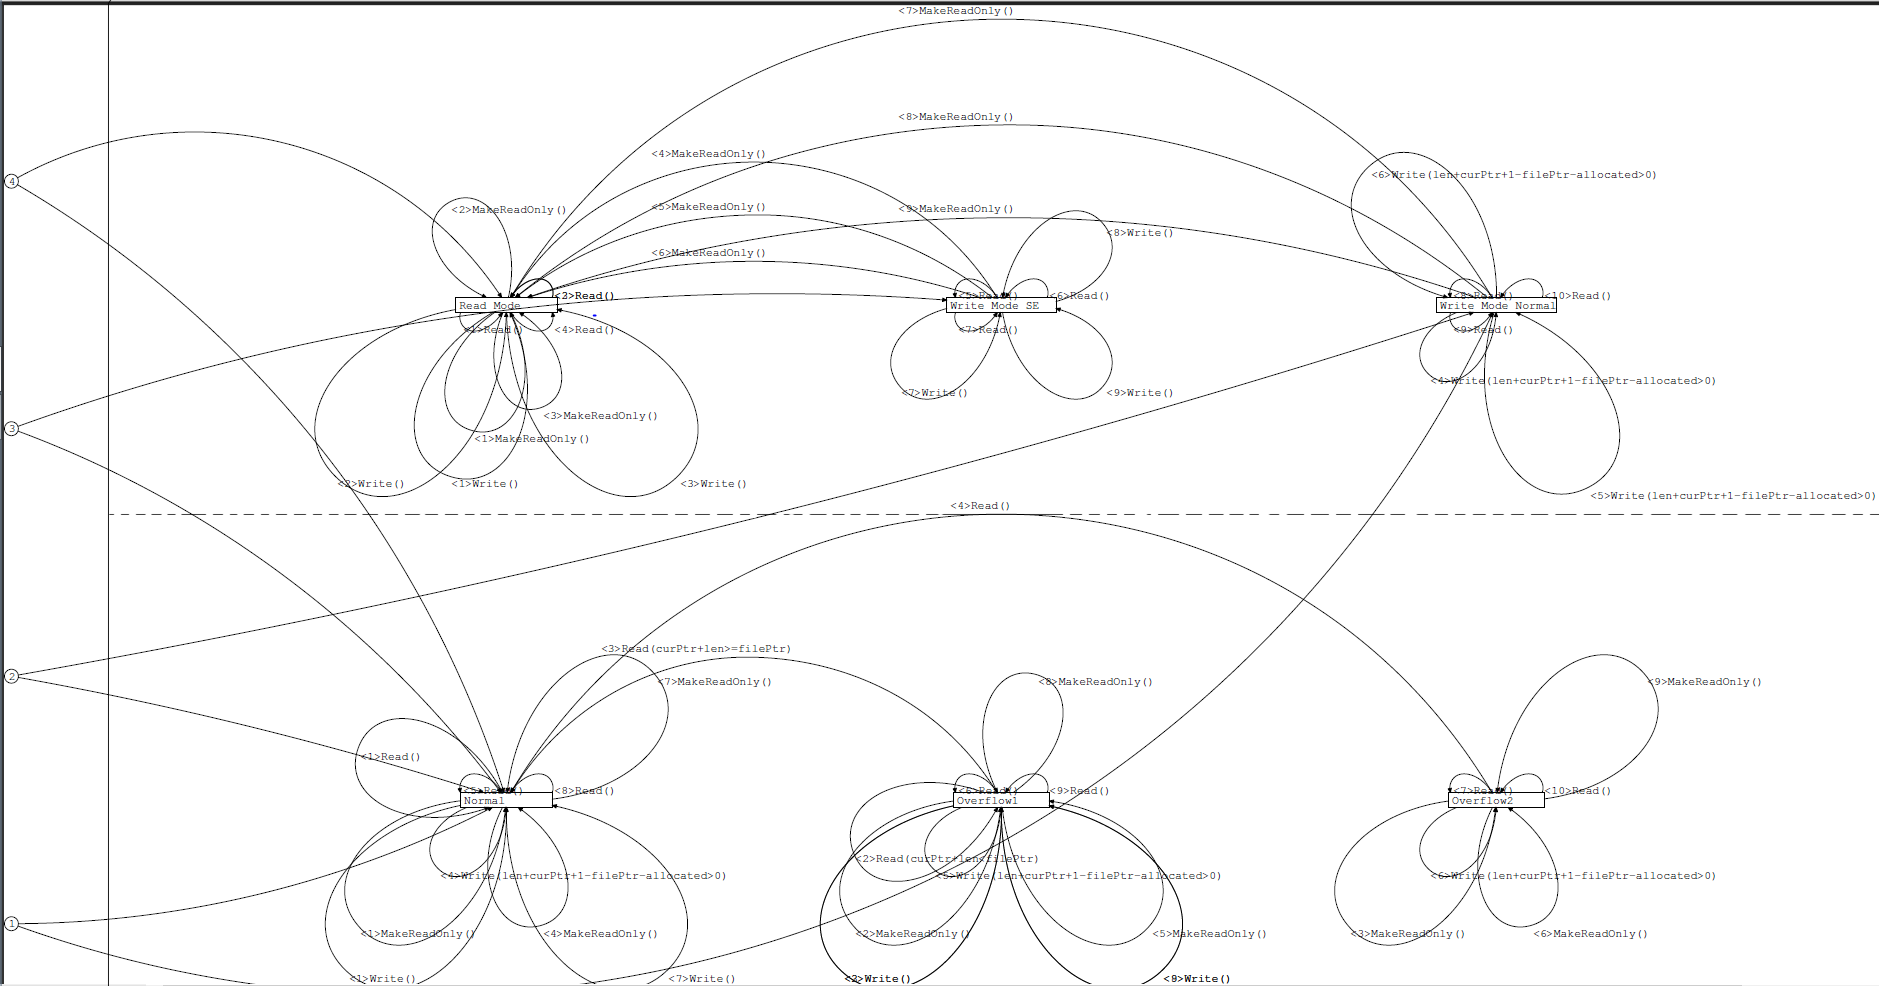
\includegraphics[width=3.5in]{img/7.PNG}
  \end{figure}
\end{frame}

\subsection{Statecharts Checking}
\begin{frame}{3 patterns of defects:}
  \begin{enumerate}
  \item Pattern 1:A state is unreachable. Defects and risks: This state cannot be a prestate of any function, thus there possibly exists defects or correctness-irrelevant redundancy. \pause
  \item Pattern 2:A common state cannot reach any common states. Defects and risks: This state is actually a exception, which should not be described as a common state in its class specification. \pause
  \item Pattern 3:There exists null-transitions. Defects and risks: Some conditions may be ignored in the class specification.
  \end{enumerate}
\end{frame}



\section{Q\&A}
\begin{frame}
  \begin{center}
    \Huge{Q \& A}
  \end{center}
\end{frame}

\end{document}

